\documentclass[11pt]{article}

\title{ECO326 Advanced Microeconomic Theory \\ \small A Course in Game Theory}

\author{Tianyu Du}
\date{\today}

\usepackage{spikey}
\usepackage{amsmath}
\usepackage{amssymb}
\usepackage{soul}
\usepackage{float}
\usepackage{graphicx}
\usepackage{hyperref}
\usepackage{xcolor}
\usepackage{chngcntr}
\usepackage{centernot}
\usepackage[shortlabels]{enumitem}
\usepackage[margin=1truein]{geometry}
\usepackage{sgame}
\usepackage{egameps}
\usepackage[perpage]{footmisc}

\counterwithin{equation}{section}
\counterwithin{figure}{section}


\newcommand{\floor}[1]{\lfloor #1 \rfloor}

\usepackage[
    type={CC},
    modifier={by-nc},
    version={4.0},
]{doclicense}

\begin{document}
	\maketitle
	\doclicenseThis
	\begin{itemize}
		\item GitHub: \url{https://github.com/TianyuDu/Spikey_UofT_Notes}
		\item Website: \url{TianyuDu.com/notes}
	\end{itemize}
	
	\tableofcontents
	\newpage
	
	\section{Lecture 1. Jan. 7 2019\\Strategic Games and Dominant Strategies}
%		\paragraph{Game Theory} Choice environment where individual choices impact others.
%		
%		\begin{example}
%			\begin{figure}[h]
%				\centering
%				  \begin{tabular}{c|c|c}
%				    & W & S\\
%				    \hline
%				    W & $(1-c, 1-c)$ & $(\red{1-c}, \red{1})$ \\
%				    \hline
%				    S & $(\red{1}, \red{1-c})$ & $(0, 0)$
%				  \end{tabular}
%				  \caption{Payoff Matrix for Example 1}
%			\end{figure}
%		\end{example}
%		Suppose $c \in (0, 1)$. In this game,
%		\begin{enumerate}[i]
%			\item $N = \{i, j\}$,
%			\item $A_i = A_j = \{W, S\}$,
%		\end{enumerate}
		
		\begin{definition}[pg.7]
			A \textbf{preference relation} is a \ul{complete reflexive and transitive} binary relation.
		\end{definition}
		
		\begin{definition}[11.1, lec.1]
			A \textbf{(strategic) game} consists of
			\begin{enumerate}[i]
				\item a \ul{finite} set of \textbf{players} $N$, with $|N| \geq 2$;
				\item for each player $i \in N$, an \textbf{action set} $A_i \neq \varnothing$;
				\item for each player $i \in N$, a \textbf{preference relation} $\succsim_i$ defined on $A := \prod_{i\in N}A_i$.
			\end{enumerate}
			and can be written as a triple $\langle N, (A_i), (\succsim_i) \rangle$.
		\end{definition}

		\begin{definition}
			An \textbf{action profile} is a $n$-tuple of actions $a_i \in A_i$ for each player $i \in N$ and denoted as 
				\begin{equation}
					(a_i)_{i \in N} \tx{ or } (a_i)
				\end{equation}
			The \textbf{action profile space} is defined as 
				\begin{equation}
					A := \prod_{i \in N} A_i
				\end{equation}
			And the space of \textbf{actions of opponents} is defined as
			\begin{equation}
				A_{-i} := \prod_{j \neq i} A_j
			\end{equation}
		\end{definition}
		
		\begin{definition}[Equivalent definition of game]
			For each player $i \in N$ we can define a \textbf{utility function}, $u_i: A \to \R$ such that
			\begin{equation}
				\forall (a_i), (a_i)' \in A,\ u_i((a_i)) \geq u_i((a_i)') \iff (a_i) \succsim_i (a_i)'
			\end{equation}
			So the game can be defined as a triple $\langle N, (A_i), (u_i) \rangle$.
		\end{definition}
		
		\begin{definition}
			Action $a_i \in A_i$ is \textbf{strictly dominated} by action $\tilde{a}_i \in A_i$ if
			\begin{equation}
				\forall a_{-i} \in A_{-i},\ u_i(a_i, a_{-i}) < u_i(\tilde{a}_i, a_{-i})
			\end{equation}
			And $a_i$ is \textbf{weakly dominated} by $\tilde{a}_i$ if
			\begin{equation}
				\forall\ a_{-i} \in A_{-i},\ u_i(a_i, a_{-i}) \leq u_i(\tilde{a}_i, a_{-i})
			\end{equation}
			\ul{and}
			\begin{equation}
				\exists\ a_{-i} \in A_{-i},\ u_i(a_i, a_{-i}) < u_i(\tilde{a}_i, a_{-i})
			\end{equation}
		\end{definition}
		
		\begin{corollary}[Consequence of RCT]
			It is irrational to play strictly dominated actions. So rational choice theory suggests a player would \ul{never} play \ul{strictly} dominated strategies.
		\end{corollary}
		
		\begin{definition}
			Action $a_i \in A_i$ is \textbf{strictly(weakly) dominant} if it strictly(weakly) dominates \ul{all} other actions.
		\end{definition}
		
		\begin{definition}
			Action $a_i \in A_i$ is \textbf{strictly(weakly) dominated} if \ul{there exists} another strategy strictly(weakly) dominates $a_i$.
		\end{definition}
		
%		\begin{example}[Prisoner Dilemma]
%			\begin{figure}[h]
%				\centering
%				\begin{tabular}{c|c|c}
%					 & S & C \\
%					\hline
%					S & (-1, -1) & (-10, \red{0})\\
%					\hline
%					C & (\red{0}, -10) & (\red{-5}, \red{-5})
%				\end{tabular}
%				\caption{Payoff matrix for example 2}
%			\end{figure}
%			Note that S is strictly dominated by C. Therefore C is strictly dominant for both players.
%		\end{example}
%		
%		\begin{example}
%			\begin{figure}[h]
%				\centering
%				\begin{tabular}{c|c|c|c}
%					 & L & C & R\\
%					\hline
%					U & (2, \red{2}) & (\red{5}, 0) & (\red{3}, 0)\\
%					\hline
%					M & (2, \red{7}) & (2, 5) & (2, 6)\\
%					\hline 
%					D & (\red{5}, \red{3}) & (4, 2) & (\red{3}, 1)
%				\end{tabular}
%				\caption{Payoff matrix for example 2}
%			\end{figure}
%			So in this game, for player 2, L is strictly dominant. \\For player 1, M is strictly dominated by D. And M is weakly dominated by U.
%		\end{example}
		
		% \begin{example}
		% 	There are three candidates, $\{A, B, C\}$. And there are 50 players (voters, note that $\varnothing \notin A_i$ since they must vote).
		% 	And 
		% 	\begin{equation}
		% 		\forall i \in N,\ A_i = \{A, B, C\}
		% 	\end{equation}
		% 	Each individual has strictly preference over $A, B, C$. If tie is encountered, randomization would be taken.
		% 	\begin{enumerate}[i]
		% 		\item $A \succ B \succ C$,
		% 		\item $A \succ AC_{tie} \succ C$
		% 	\end{enumerate}
		% 	\paragraph{Claim 1:}There are no weakly or strictly dominant actions. 
		% 	\begin{proof}
		% 		Let $a_i \in \{V_A, V_B, V_C\}$ denote the action taken by player $i \in N$, \\
		% 		Note that weak dominance is a necessary condition for strict dominance, \\
		% 		So above claim is reduced to \emph{there are no weakly dominant actions}. \\
		% 		The reduced claim is equivalent to the following statement, \\
				
		% 		\begin{gather*}
		% 			\forall a_i \in A_i,\ \exists \tilde{a}_i \in A_i\ s.t.\ a_i \neq \tilde{a}_i\\
		% 			s.t.\ \exists a_{-i} \in A_{-i}\ s.t.\ u_i(a_i, a_{-i}) > u_i(\tilde{a}_i, a_{-i}) \lor \forall a_{-i} \in A_{-i},\ u_i(a_i, a_{-i}) = u_i(\tilde{a}_i, a_{-i})
		% 		\end{gather*}
		% 		Let $n_{-i}^j$ denote the number of voters other than $i$ voting for candidate $j$. Clearly each $a_{-i} \in A_{-i}$ would induce an outcome as a triple $(n_{-i}^A, n_{-i}^B, n_{-i}^C)$.\\
		% 		Consider action $V_A$, and $a_{-i}$ induces 
		% 		\begin{equation}
		% 			(n_{-i}^A, n_{-i}^B, n_{-i}^C) = (1, 24, 24)
		% 		\end{equation}
		% 		then 
		% 		\begin{equation}
		% 			(V_B, a_{-i}) \succ_i (V_A, a_{-i})
		% 		\end{equation}
		% 		So $V_A$ failed to be a dominant strategy of any kind. \\
		% 		Similarly, consider action $V_B$, if $a_{-i}$ induces
		% 		\begin{equation}
		% 			(n_{-i}^A, n_{-i}^B, n_{-i}^C) = (24, 1, 24)
		% 		\end{equation}
		% 		then 
		% 		\begin{equation}
		% 			(V_A, a_{-i}) \succsim_i (V_B, a_{-i})
		% 		\end{equation}
		% 		So $V_B$ failed to be a dominant strategy. \\
		% 		Similarly, consider action $V_C$, if $a_{-i}$ induces
		% 		\begin{equation}
		% 			(n_{-i}^A, n_{-i}^B, n_{-i}^C) = (24, 24, 1)
		% 		\end{equation}
		% 		then 
		% 		\begin{equation}
		% 			(V_A, a_{-i}) \succsim_i (V_C, a_{-i})
		% 		\end{equation}
		% 		So $V_B$ failed to be a dominant strategy.
		% 	\end{proof}
		% 	\paragraph{Claim 2:}Only voting for your least preferred candidate is weakly dominated.
		% 	\begin{proof}
		% 		We are going to show there exists a strategy (voting for $B$) weakly dominates voting for $C$.
		% 		\begin{figure}[H]
		% 			\centering
		% 			\begin{tabular}{c|c|c}
		% 				Vote A & Cases & Vote C \\
		% 				\hline
		% 				A & $n_{-i}^A > n_{-i}^B, n_{-i}^C$ & A, AC \\
		% 				B & $n_{-i}^B > n_{-i}^A, n_{-i}^C$ & B, BC \\
		% 				C, BC & $n_{-i}^C > n_{-i}^A, n_{-i}^B$ & C\\
		% 				B & $n_{-i}^A = n_{-i}^B > n_{-i}^C$ & AB\\
		% 				A & $n_{-i}^A = n_{-i}^C > n_{-i}^B$ & C\\
		% 				BC & $n_{-i}^C = n_{-i}^B > n_{-i}^A$ & C
		% 			\end{tabular}
		% 			\caption{Voting for A versus Voting for C}
		% 		\end{figure}
		% 	\end{proof}
		% \end{example}
		
		\begin{definition}
			A strategic game $\langle N, (A_i), (\succsim_i) \rangle$ is \textbf{finite} if for every $i \in N$, $A_i$ is finite.
		\end{definition}
	
	\section{Lecture 2. Jan. 14 2019\\Iterated Elimination and Rationalizability}
%		\begin{example}[Bubble Game]
%			Consider a strategic game
%			\begin{equation}
%				\langle N, (A_i), (u_i) \rangle
%			\end{equation}
%			where 
%			\begin{equation}
%				A_i = \{0,\dots,100\},\ \forall i
%			\end{equation}
%			and 
%			\begin{gather}
%				u_i(a_i, a_{-i}) = a_i - penalty_i(a_i, a_{-i}) \\
%				penalty_i = \begin{cases}
%					0 &\tx{ if } a_i < \max_{j \neq i} a_j - 1 \\
%					10(a_i - \max_{j \neq i} a_j + 1) &\tx{ if } a_i \geq \max_{j \neq i} - 1
%				\end{cases}
%			\end{gather}
%		\end{example}	
		
		\subsection{Iterated Elimination of Strictly Dominated Strategies/Actions}
			\begin{definition}[IESD]
				Given the initial game,
				\begin{equation}
					G_0 = \langle N, (A^0_i), (u_i) \rangle
				\end{equation} 
				At stage $k \in \N$, 
				\begin{equation}
					G_k = \langle N, (A^k_i), (u_i) \rangle
				\end{equation}
				In stage $k$, for all $i \in N$, find the set of \ul{strictly} dominated actions, $D_i^k \subsetneq A_i^k$.
				\begin{enumerate}[i)]
					\item If $\forall i \in N\ s.t.\ D_i^k = \varnothing$, conclude the profile
					\begin{equation}
						(A_i^k)
					\end{equation}
					to be the \textbf{set of action profiles survive from IESD}.
					\item If $\exists i \in N\ s.t.\ D_i^k \neq \varnothing$, define
					\begin{equation}
						\forall i \in N,\ A^{k+1}_i \leftarrow A^k_i \backslash D_i^k
					\end{equation}
				\end{enumerate}
			\end{definition}
			
%			\begin{example}
%				Action profile $(M, R)$ survives the IESD.
%				\begin{proof}
%					\begin{gather*}
%						k=0,\ A_1^0 = \{U, M, D\},\ 
%						A_2^0 = \{L, R\} \\
%						k=1,\ A_1^1 = \{U, M\},\ 
%						A_2^1 = \{L, R\} \\
%						k=2,\ A_1^2 = \{U, M\},\ 
%						A_2^2 = \{R\} \\
%						k=3,\ A_1^3 = \{M\},\ 
%						A_2^3 = \{R\} \\
%					\end{gather*}
%				\end{proof}
%			\end{example}
%			\begin{figure*}[h]
%				\centering
%				\begin{tabular}{l|cc}
%				  & L & R \\
%				  \hline
%				  U & 4,0 & 2,2 \\
%				  M & 1, 2& \red{5,3} \\
%				  D & 0,5 & 1,4 \\
%				\end{tabular}
%			\end{figure*}
			
			\begin{example}[Hotelling Model of Politics]
				Players maximize their votes by choosing where to stand along a natural number line.
				\begin{itemize}
					\item Player $N = \{1,2\}$
					\item Action set $A_i = \{1, \dots, M\}$, with $2 \centernot | M$ and $M > 3$.
					\item Payoff
					\begin{equation}
						u_i(a_i, a_{-i}) = \begin{cases}
							a_i + \frac{1}{2}(a_{-i} - a_{i} - 1) \tx{ if } a_i < a_{-i} \\
							\frac{M}{2} \tx{ if } a_i = a_{-i} \\
							M - [a_{-i} + \frac{1}{2}(a_{i} - a_{-i} - 1)] \tx{ if } a_i > a_{-i}
						\end{cases}
					\end{equation}
				\end{itemize}
				\paragraph{Claim i.} $a_i=1$ is strictly dominated by $a_i=2$.
				\begin{proof}
					\begin{gather}
						u_i(a_i=1, a_{-i}) =
						\begin{cases}
							\frac{M}{2} \tx{ if } a_{-i} = 1 \\
							\frac{a_{-i}}{2} \tx{ if } a_{-i} > 1
						\end{cases} \\
						u_i(a_i=2, a_{-i}) = 
						\begin{cases}
							M - 1 \tx{ if } a_{-i} = 1 \\
							\frac{M}{2} \tx{ if } a_{-i} = 2 \\
							\frac{a_{-i}}{2} + \frac{1}{2} \tx{ if } a_{-i} > 2
						\end{cases}
					\end{gather}
				\end{proof}
				\paragraph{Claim ii.} $\floor{\frac{n}{2}} + 1$ is the only action survives.
				\begin{proof}
					Similarly, we can eliminate all edge-values iteratively.
				\end{proof}
			\end{example}
			
			\begin{definition}
				For each $i \in N$, the \textbf{best-response function} of this player is a correspondence $Br_i: A_{-i} \rightrightarrows A_i$ defined as
				\begin{equation}
					Br_i(a_{-i}) := \{a_i \in A_i : u_i(a_i, a_{-i}) \geq u_i(a_i', a_{-i})\ \forall a_i' \in A_i \}
				\end{equation}
			\end{definition}
			
			\begin{definition}
				A \textbf{belief} of player $i$ (about the actions of the other players) is a \ul{probability measure}, $\alpha_i \in \Delta(A_{-i})$.
%				$\alpha_i$ is a mapping such that
%				\begin{itemize}
%					\item $\alpha_i: A_{-i} \to [0,1]$.
%					\item $\alpha_i(A_{-i}) = 1$.
%					\item For all countable piece-wise \ul{disjoint} collection 
%					\begin{equation}
%						\{E_j\}_{j\in \mc{J}} \in \mc{P}(A_{-i})
%					\end{equation}
%					$\alpha_i$ satisfies the \emph{countable additivity property}:
%					\begin{equation}
%						\alpha_i(\bigcup_{i \in I} E_i) = \sum_{i \in I}\alpha_i(E_i)
%					\end{equation}
%				\end{itemize}
			\end{definition}
			
%			\begin{remark}
%				$\alpha_i$ defines a distribution of $a_{-i}$.
%			\end{remark}
			
			\begin{definition}
				$a_i$ is a \ul{\textbf{best response} to the belief $\alpha_i$} if
				\begin{equation}
					\forall a_i' \in A_i,\ \sum_{a_{-i} \in A_{-i}} u_i(a_i, a_{-i}) \alpha_i(a_{-i}) \geq \sum_{a_{-i} \in A_{-i}} u_i(a_i', a_{-i}) \alpha_i(a_{-i})
				\end{equation}
				more precisely,
				\begin{equation}
					\forall a'_i \in A_i,\ \expect{u_i(a_i, a_{-i})|\alpha_i} \geq \expect{u_i(a_i', a_{-i})|\alpha_i}
				\end{equation}
			\end{definition}
			
			\begin{definition}
				$a_i \in A_i$ is a \textbf{never best response} if it is not a best response given any belief $\alpha_i$.
			\end{definition}
			
			\begin{corollary}
				[\emph{Iterative Elimination of Never Best Response}] Same procedures but $D_i^k$ is the set of never best responses for player $i$ at game $G^k$.
			\end{corollary}
			
			\begin{example}
				For player 1, $D$ is not strictly dominated, but it is a never best response.
				\begin{proof}
					Let $\alpha$ be a probability measure on $\{L, R\}$ such that $\alpha(L) = p \in [0, 1]$.\\
					\begin{align}
						\expect{u_1(U)|\alpha} &= 10p \\
						\expect{u_1(M)|\alpha} &= 10 - 10p \\
						\expect{u_1(D)|\alpha} &= 1
					\end{align}
					\textbf{Case i}
					\begin{equation}
						p \geq 0.5 \implies \expect{u_1(U)|\alpha} \geq 5 > \expect{u_1(D)|\alpha}
					\end{equation}
					\textbf{Case ii}
					\begin{equation}
						p < 0.5 \implies \expect{u_1(M)|\alpha} > 5 > \expect{u_1(D)|\alpha}
					\end{equation}
					Therefore, for any belief $\alpha$, $D$ cannot be a best response. So $D$ is a never best response.
				\end{proof}
			\end{example}
			\begin{figure}[h]
				\centering
				\begin{tabular}{l|cc}
				  & L & R\\
				  \hline
				  U & 10,0 & 0,0 \\
				  M & 0,0 & 10,0\\
				  D & 1,0 & 1,0
				\end{tabular}
			\end{figure}
			
			\begin{definition}
				An action $a_i \in A_i$ is \textbf{rationalizable} if it survives \emph{iterative elimination of never best responses} (i.e. action $a_i$ is a best response to some mixed strategies of opponents).
			\end{definition}
			
			\begin{lemma}[60.1]
				An action of a player in a \emph{finite} strategic game is a never-best response \emph{if and only if} it is strictly dominated. \footnote{The concept of \emph{strict domination} will be introduced in section 5.}
			\end{lemma}
		
	\section{Lecture 3. Jan. 21 2019\\Pure Strategy Nash Equilibrium}
		\begin{definition}
			A \textbf{pure strategy Nash equilibrium} is an \ul{action profile} $(a_i)$ such that 
			\begin{equation}
				\forall i \in N,\ a_i \in Br_i(a_{-i})
			\end{equation}
		\end{definition}
			
		\begin{remark}
			That's, a NE is a situation that if player $i$ knows what other players do, there exists no beneficial deviation from the current strategy.
		\end{remark}
		
		\begin{remark}[Interpretations]
			A Nash equilibrium is 
			\begin{enumerate}[i)]
				\item An action profile induces a \ul{stable outcome},
				\item A \ul{creditable agreement}, such that no player has incentive to break the agreement.
			\end{enumerate}
		\end{remark}
		
		\begin{example}[Cournot Duopoly]
			Consider a game with
			\begin{enumerate}[i)]
				\item Player $N = \{1,2\}$
				\item Action set $A_i = [0, \infty)\ \forall i \in N$
			\end{enumerate}
			And revenue $R_i$ defined by 
			\begin{equation}
				R_i = p_i q_i
			\end{equation}
			where price is linear in quantity supplied,
			\begin{equation}
				p_i = \alpha - (q_i + q_{-i}),\ \alpha \in \R
			\end{equation}
			and firms face fixed cost $c \in \R$, with the assumption that $\alpha > c$. So the cost function is given by
			\begin{equation}
				C_i(q_i) = c q_i 
			\end{equation}
			The profit function is given by
			\begin{gather}
				\Pi_i(q_i, q_{-i}) = (\alpha - (q_i + q_{-i}) - c) q_i \\
				= (\alpha-c-q_{-i})q_i - q_i^2
			\end{gather}
			Given $q_{-i} \in A_{-i}$, the best response is given by
			\begin{gather}
				Br_i(q_{-i}) = \tx{argmax}_{q_i \in [0, \infty)} \Pi_i(q_i, q_{-i}) \\
				= \max\{0, \frac{\alpha - c - q_{-i}}{2}\}\ \forall i \in N
			\end{gather}
			Considering the case that both players are producing positive quantities, we can solve $q_i^*$ by
			\begin{gather}
				Br_i \circ Br_{-i}(q_i) = \frac{\alpha - c - \frac{\alpha - c - q_i}{2}}{2} = q_i \\
				\implies 2 q_i - \frac{q_i}{2} = \frac{\alpha - c}{2} \\
				\implies q_i^* = \frac{\alpha - c}{3}
			\end{gather}
			
			\begin{remark}
				If fixed cost presents, even if the game is symmetric, the Nash equilibrium could be asymmetric. (e.g. one firm is out of market and the other firm produces the monopoly amount)
			\end{remark}
		\end{example}
		
		\begin{remark}
			Nash equilibrium induces an \emph{individual level optimality} instead of the common wealth optimality.
		\end{remark}
		
		\begin{example}[Continue Cournot Duopoly]
			Note that in the Cournot Duopoly game, for each $i \in N$, the Nash equilibrium profit is
			\begin{gather}
				\Pi_{NE}^* = \left(\alpha - c - \frac{2(\alpha - c)}{3}\right) \frac{\alpha - c}{3} \\
				= \frac{(\alpha - c)^2}{9}
			\end{gather}
			So the total profit for the two firms is $\frac{2(\alpha - c)^2}{9}$. \\
			Now considering if the two firms form a Cartel, the \emph{aggregate} quantity produced is
			\begin{gather}
				Q^* = \tx{argmax}_{Q \in \R_{\geq 0}} (\alpha - c - Q) Q \\
				= \frac{\alpha - c}{2} \\
				\implies \Pi_{Cartel}^* = \left(\alpha - c - \frac{\alpha - c}{2} \right)\frac{\alpha - c}{2} \\
				= \frac{(\alpha - c)^2}{4} > \frac{2(\alpha - c)^2}{9}
			\end{gather}
			The fact $\Pi_{Cartel}^* > 2 \times \Pi_{NE}^*$ suggests the Nash equilibrium action profile did not induce the optimal common wealth outcome. However, the Cartel action profile is not a stable outcome since every player has incentive to increase their production level.
		\end{example}
		
		\begin{example}[Prisoner's Dilemma]
			The Nash equilibrium(Confess, Confess) is \ul{not} the best outcome for the two players as a group. The optimal action profile \ul{for a group} is (Silent, Silent).
		\end{example}
		
		\begin{proposition}
			No strategy that is eliminated during iterated elimination of \emph{never best response} can be played in a Nash equilibrium.
		\end{proposition}
	
	\section{Lecture 4. Jan. 28. 2019\\Nash Equilibrium: Examples}
	\begin{example}[From last lecture]
		Consider the payoff matrix
		\begin{figure*}[h]
			\centering
			\begin{tabular}{c|c|c}
				 & A & B \\
				\hline
				A & (\red{1},\red{1}) & (\red{0},0) \\
				B & (0,\red{0}) & (\red{0},\red{0}) \\
			\end{tabular}
		\end{figure*}
		Both $(A,A)$ and $(B,B)$ are Nash equilibria. But in the former NE, for each $i \in N$,
		\begin{equation}
			Br_i(a_{-i}=A) = \{A\}
		\end{equation}
		which is a singleton. \\
		In the second NE, for each $i \in N$,
		\begin{equation}
			Br_i(a_{-i}=B) = \{A, B\}
		\end{equation}
		We call Nash equilibria of the first type \emph{strict Nash equilibria} and the later one \emph{weak Nash equilibria}. More formal definitions of these two types of Nash equilibria are given below.
	\end{example}
	
	\begin{definition}
		A \textbf{strict Nash equilibrium} is an action profile $(a_i)$ such that
		\begin{equation}
			\forall i \in N,\ Br_i(a_{-i}) \tx{ is a singleton.}
		\end{equation}
	\end{definition}
	
	\begin{definition}
		A \textbf{weak Nash equilibrium} is a Nash equilibrium that is not strict.
	\end{definition}
	
	\begin{example}[Cournot with $n$ firms]
		Consider the game 
		\begin{equation}
			\langle N, (\R_{\geq 0}), (\pi_i) \rangle
		\end{equation}
		Where $|N| = n$ and each firm picks a quantity $q_i \in A_i := \R_{\geq 0}$. \\
		Define 
		\begin{equation}
			Q := \sum_j q_j
		\end{equation}
		For each $i \in N$, define 
		\begin{equation}
			Q_{-i} := \sum_{j\neq i} q_j
		\end{equation}
		And the market has \emph{linear demand curve}
		\begin{equation}
			P(\{q_i\}_{i\in N}) = \alpha - \sum_{j}q_j = \alpha - Q
		\end{equation}
		And firms face fixed cost
		\begin{equation}
			\forall i \in N,\ C(q_i) = c q_i \tx{ where } 0 < c < \alpha
		\end{equation}
		The profit function is
		\begin{equation}
			\forall i \in N,\ \pi_i(q_i, Q_{-i}) = (\alpha - c - Q_{-i})q_i - q_i^2
		\end{equation}
		\paragraph{Question}What are the Nash equilibria in this environment? \\
		For each firm $i \in N$, the best response correspondence is
		\begin{gather}
			Br_i(Q_{-i}) = \max\{0, \argmax_{q_i \in \nnr} \pi_{i}(q_i, Q_{-i}) \} \\
			= \max\{0, \frac{\alpha - c - Q_{-i}}{2}\}
		\end{gather}
		\paragraph{Assume}We have a symmetric Nash equilibrium, 
		\begin{gather}
			\forall i \in N,\ q^*_i = q^* = \frac{Q}{n} \\
			\implies q^* = Br_i(\frac{n-1}{n}Q) \\
			\implies 2 q^* = \alpha - c - (n-1) q^* \\
			\implies q^* = \frac{\alpha - c}{n + 1}
		\end{gather}
		\paragraph{Check}Then check the validity of symmetric Nash equilibrium by asserting for every player, if all other players are playing the action suggested by the symmetric Nash equilibrium, then this player should also play it. That's
		\begin{gather}
			q^* = Br_i(\{q_j\}_{j\neq i}) \\
			= \frac{\alpha - c}{2} - \frac{1}{2} \frac{n-1}{n+1} (\alpha - c) \\
			= \frac{1}{2}((\alpha - c) - \frac{n-1}{n+1}(\alpha - c)) \\
			= \frac{1}{2} \frac{2}{n+1}(\alpha - c) \\
			= \frac{\alpha - c}{n + 1} 
			= q^*
		\end{gather}
		\paragraph{Uniqueness} We are going to show the symmetric Nash equilibrium is the only possible equilibrium action profile. \\
		\begin{proof}
			Suppose there exists some non-symmetric Nash equilibrium. \\
			For concreteness, assuming there exists $\epsilon > 0$ such that
			\begin{equation}
				\exists i, j \in N,\ q_i = q_j + \epsilon
			\end{equation}
			Define $Q_{-ij} := Q - q_i - q_j$.\\
			For firm $i$,
			\begin{gather}
				q_i = Br_i(Q_{-i}) = \frac{1}{2} (\alpha - c - Q_{-i}) \\
				= \frac{1}{2}(\alpha - c - Q_{-ij} - q_{j}) \\
				= \frac{1}{2}(\alpha - c - Q_{-ij} - q_i + \epsilon) \\
				\implies 3 q_i = \alpha - c - Q_{-ij} + \epsilon \\
				\implies 3 q_i = \alpha - c - Q_{-j} + q_i + \epsilon \\
				\implies 2 q_i - \epsilon = \alpha - c - Q_{-j} \\
				\implies  q_i - \frac{\epsilon}{2} = Br(Q_{-j}) = q_j \\
				= q_i - \epsilon \\
				\implies \epsilon = 2 \epsilon
			\end{gather}
			which contradicts the assumption that $\epsilon > 0$. \\
			Therefore we conclude that the symmetric Nash equilibrium is the only Nash equilibrium in this environment.
		\end{proof}
	\end{example}
	
	\begin{example}[Cournot duopoly with fixed cost]
		Consider the game 
		\begin{equation}
			\mc{G} = \langle N = (1,2), (A_i = \nnr), (\pi_i) \rangle
		\end{equation}
		Where the cost function is defined as
		\begin{equation}
			C_i(q_i) = \begin{cases}
				c q_i + f &\tx{ if } q_i > 0 \\
				0 &\tx{ if } q_i = 0
			\end{cases}
		\end{equation}
		where $\alpha > c > 0$. \\
		For each firm $i \in N$, the best response function, conditioned on $q_i > 0$, is
		\begin{equation}
			q_i = Br_i(q_{-i}) = \frac{\alpha - c - q_{-i}}{2}
		\end{equation}
		We have to \textbf{check the profit} to assert the profit is non-negative while firm $i$ is producing above quantity. Because, otherwise, this firm could always derivate to $q_i = 0$ to avoid loss (earning zero profit).
		\begin{gather}
			\pi_i(Br_{q_{-i}}, q_{-i}) = (\alpha - q_{-i} - \frac{\alpha - c - q_{-i}}{2} - c)\frac{\alpha - c - q_{-i}}{2} - f \\
			= \frac{(\alpha - c - q_{-i})^2}{4} - f \\
			\pi_i(q_{-i}) \geq 0 \iff \alpha - c - q_{-i} \geq 2\sqrt{f} \\
			\iff q_{-i} \leq \alpha - c - 2\sqrt{f}
		\end{gather}
		Therefore we can modify our \textbf{best response correspondence} to
		\begin{gather}
			Br_i(q_{-i}) = 
			\begin{cases}
				\frac{\alpha - c - q_{-i}}{2} &\tx{ if }  q_{-i} \leq \alpha - c - 2\sqrt{f} \\
				0 &\tx{ if } q_{-i} \geq \alpha - c - 2\sqrt{f}
			\end{cases}
		\end{gather}
		\textbf{Monopoly}: the monopoly amount, conditioned on the firm decides to produce, is $\frac{\alpha - c}{2}$. In the monopoly case, suppose the NE action profile is (the opposite case can be shown by symmetry)
		\begin{equation}
			(\frac{\alpha - c}{2}, 0)
		\end{equation}
		We have to assert both 
		\begin{gather}
			\begin{cases}
				\frac{\alpha - c}{2} \in Br_1(0) \\
				0 \in Br_2(\frac{\alpha - c}{2})
			\end{cases} \\
			\implies
			\begin{cases}
				0 \leq \alpha - c - 2\sqrt{f} &\tx{ for firm 1 to produce positive amount.}\\
				\frac{\alpha - c}{2} \geq \alpha - c - 2\sqrt{f} &\tx{ for firm 2 to produce zero.}
			\end{cases} \\
			\implies 0 \leq \alpha - c - 2\sqrt{f} \leq \frac{\alpha - c}{2} \\
			\implies -(\alpha - c) \leq - 2\sqrt{f} \leq -\frac{\alpha - c}{2} \\
			\implies \red{\sqrt{f} \in [\frac{\alpha-c}{4}, \frac{\alpha - c}{2}]}
		\end{gather}
		\textbf{Positive symmetric equilibrium}: we've proven, in the general case, it's impossible for both firms to produce positive but different amounts. Therefore we have to assert 
		\begin{gather}
			\frac{\alpha - c}{3} \in Br_i(\frac{\alpha - c}{3})\ \forall i \in N \\
			\implies \frac{\alpha - c}{3} \leq \alpha - c - 2\sqrt{f} \\
			\implies \sqrt{f} \leq \frac{1}{3} (\alpha - c)
		\end{gather}
		\textbf{Zero symmetric equilibrium}: we have to assert
		\begin{gather}
			0 \in Br_i(0)\ \forall i \in N\\
			\implies 0 \geq \alpha - c - 2\sqrt{f} \\
			\implies \sqrt{f} \geq \frac{\alpha - c}{2}
		\end{gather}
	\end{example}
	
	\begin{example}[Discrete price Bertrand duopoly]
		Consider the following game
		\begin{gather}
			\mc{G} = \langle N=\{1,2\}, (A_i = \{k \epsilon: k \in \Z_{\geq 0}\}), (\pi_i) \rangle
		\end{gather}
		The profit function can be derived as
		\begin{gather}
			\pi_i(p_i, p_{-i}) = \begin{cases}
				(\alpha - p_i)(p_i - c)&\tx{ if } p_i < p_{-i} \\
				\frac{\alpha - p_i}{2}(p_i - c) &\tx{ if } p_i = p_{-i} \\
				0 &\tx{ if } p_i > p_{-i}
			\end{cases}
		\end{gather}
		\textbf{Claim} the only Nash equilibria are $(c, c)$ and $(c+\epsilon, c+\epsilon)$. \\
		\textbf{Justify} $(c, c)$, consider any firm $i \in N$, currently $\pi_i = 0$ 
		\begin{gather}
			\uparrow p_i \implies \pi_i \leftarrow \pi_i' = 0 \tx{ \xmark} \\
			\downarrow p_i \implies \pi_i \leftarrow \pi_i' < 0 \tx{ \xmark}
		\end{gather}
		So no firm has incentive to derivate from this action profile, so $(c, c)$ is a Nash equilibrium by definition. \\
		Consider the action profile $(c+\epsilon, c+\epsilon)$, both firms are earning a positive profit $\pi_i > 0$. For any firm $i \in N$,
		\begin{gather}
			\uparrow p_i \implies \pi_i \leftarrow \pi_i' = 0 \tx{ \xmark} \\
			\downarrow p_i \implies \pi_i \leftarrow \pi_i' = 0 \tx{ \xmark}
		\end{gather}
		So $(c+\epsilon, c+\epsilon)$ is a Nash equilibrium by definition. \\
		\textbf{No other Nash equilibrium} \\
		\textbf{Claim}: $(p_1, p_2)$ cannot be a Nash equilibrium if any $p_i < c$. \\
		Obviously, set $p_i < c$ would induce negative profit and firm $i$ do better off by setting $p_i \leftarrow c$. \\
		\textbf{Claim}: the symmetric profit $(p, p)$ with $p > c + \epsilon$ cannot be a Nash equilibrium. For both firms, the current profit is
		\begin{equation}
			\pi_1 = \pi_2 = \frac{1}{2}(\alpha - c - k\epsilon) k \epsilon
		\end{equation}
		And reducing price by $\epsilon$ leads to a profit of
		\begin{equation}
			\pi_i ' = (\alpha - c - k \epsilon + \epsilon) (k-1)\epsilon > \pi_i
		\end{equation}
		so such action profile cannot be Nash equilibrium. \\
		\textbf{Claim} $(p_1, p_2)$ with $p_1 \neq p_2$ and $p_1, p_2 > c$ cannot be a Nash equilibrium. The firm charges higher price can always reduce it's price to the price charged by the other firm and gain a positive profit. \\
		\textbf{Claim} $(c, p_2)$ with $p_2 \geq c + \epsilon$ cannot be a Nash equilibrium. The firm charging $p = c $ can always increase its price to $c + \epsilon$ to earn positive profit. \\
		Therefore there's no Nash equilibrium other than $(c,c)$ and $(c+\epsilon, c+\epsilon)$.
	\end{example}
	
	\begin{example}[Bertrand duopoly with differentiated products]
		Consumers are \ul{uniformly distributed} on a preference line $[0,1]$.\\
		For a firm $i \in N$, let $x_i \in [0,1]$ measure consumer's preference towards firm $i$'s products. \\
		Define 
		\begin{equation}
			x_{-i} := 1 - x_i \sim Unif(0,1)
		\end{equation}
		Consumer buy product $i$ if 
		\begin{gather}
			x_i - p_i \geq x_{-i} - p_{-i}
		\end{gather}
		and purchases product 1 if
		\begin{gather}
			x_i - p_i \leq x_{-i} - p_{-i}
		\end{gather}
		Then solve the boundary $x^* \in [0, 1]$ such that consumers at $x^*$ are indifferent between  two products.
		\begin{gather}
			x + p_i = (1 - x) + p_{-i} \\
			\implies x^* = \frac{1 - p_i + p_{-i}}{2}
		\end{gather}
		So any consumer with $x_i > x^*$ would choose firm $i$'s product, also because consumers are uniformly distributed on $x_i \in [0,1]$. So the portion of consumers buying firm $i$'s product is
		\begin{equation}
			1 - x_i = \frac{1 + p_i - p_{-i}}{2}
		\end{equation}
		And, clearly, 
		The demand function for firm $i$ is
		\begin{gather}
			D_i(q_i, q_{-i}) = \begin{cases}
				0 &\tx{ if } p_i \geq p_{-i} + 1 \\
				\frac{1 + p_i - p_{-i}}{2} &\tx{ if } p_i \in [p_{-i}-1, p_{-i}+1]\\
				1 &\tx{ if } p_i \leq p_{-i} - 1\\
			\end{cases}
		\end{gather}
		Consider the case where $|p_i - p_{-i}| \leq 1$, 
		\begin{gather}
			\pi_i = D_i(p_i) (p_i - c) = \frac{1 + p_i - p_{-i}}{2} (p_i - c)
		\end{gather}
		Take the first order condition
		\begin{gather}
			\pd{\pi_i}{p_i} = 0 \\
			\implies p_i = \frac{p_{-i} + c - 1}{2}
		\end{gather}
	\end{example}
	
	\section{Lecture 5 Feb. 7 2019\\Mixed Strategies}
		\subsection{Lecture Contents}
%		\begin{example}Matching pennies: an example of game without pure strategy Nash equilibrium.
%			\begin{figure}[h]
%				\centering
%				\begin{game}{2}{2}
%					& $H$ & $T$ \\
%					$H$ & (\red{1},-1) & (-1,\red{1}) \\
%					$L$ & (-1,\red{1}) & (\red{1},-1) \\
%				\end{game}
%			\end{figure}
%		\end{example}
		
		\begin{assumption}
			We assume that the preference relation of each player $i$ satisfies the assumptions of \emph{von Neumann and Morgenstern}, so that it can be represented by the expected value of some utility function $u_i: A \to \R$.
		\end{assumption}
		
		\begin{definition}
			Suppose player $i$ has a \emph{finite} set of pure strategies $A_i$, then a \textbf{mixed strategy} $\sigma_i \in \Delta (A_i)$ is a probability distribution over $A_i$.
		\end{definition}
		
		\begin{definition}
			The \textbf{support} of $\sigma_i$ is defined as
			\begin{equation}
				\mc{S}(\sigma_i) := \{a \in A_i: \sigma_i(a) > 0\}
			\end{equation}
		\end{definition}
		
		\begin{definition}
			A mixed strategy $\sigma_i$ is \textbf{degenerate} if 
			\begin{equation}
				\exists a_i \in A_i\ s.t.\ \sigma_i(a_i) = 1
			\end{equation}
			and such degenerated mixed strategy is denoted as $e(a_i)$.
		\end{definition}
		
		\begin{remark}
			A pure strategy $a_i \in A_i$ is equivalent to a degenerated mixed strategy $e(a_i)$.
		\end{remark}
		
		\begin{proposition}
			In a finite game, given the independence of randomization, the probability of the action profile $a := (a_i)$ to be realized given mixed strategy profile $\sigma := (\sigma_i)$ is
			\begin{equation}
				\sigma (a) := \prob{a|\sigma} = \prod_{i \in N} \sigma_i(a_i)
			\end{equation}
			and for player $i$, the \textbf{expected payoff} from mixed strategy profile $(\sigma_i)$ is 
			\begin{equation}
				U_i(\sigma_{i}, \sigma_{-i}) := 
				\sum_{a \in A} \underbrace{\prod_{j \in N} \sigma_j(a_j)}_{\prob{a|\sigma}} u_i(a) = \expect{u_i|\sigma}
			\end{equation}
		\end{proposition}
		
		\begin{proposition}
			The \textbf{expected payoff} from mixed strategy profile $(\sigma_i) := (\sigma_i, \sigma_{-i})$ is
			\begin{equation}
				U_i(\sigma_i, \sigma_{-i}) := \expect{u_i(a)|(\sigma_i)} = \sum_{a_i \in A_i} \sum_{a_{-i} \in A_{-i}} u_i(a_i, a_{-i}) \sigma_{-i}(a_{-i}) \sigma_i(a_i)
			\end{equation}
		\end{proposition}
		
		\begin{definition}[Osborne 2030 lec2]
			The \textbf{mixed extension} of the strategic game $\langle N, (A_i)_{i\in N}, (u_i)_{i\in N} \rangle$ is the following strategic game:
			\begin{enumerate}[(i)]
				\item \textbf{Players} $N$;
				\item \textbf{Action sets} $\Delta(A_i)$ for player $i$;
				\item \textbf{Preferences} represented by $U_i: \prod_{j \in N} \Delta(A_j) \to \R$, where $U_i(\alpha)$ is the \ul{expected value} under $u_i$ of the lottery over $\prod_{j \in N} \Delta(A_j)$ induced by mixed strategy profile $\sigma \in \Delta(A)$.
			\end{enumerate}
		\end{definition}
		
		\begin{definition}
			A pure strategy $a_i \in A_i$ is \textbf{strictly dominated} by a mixed strategy $\sigma_i \in \Delta(A_i)$ if
			\begin{equation}
				\forall a_{-i} \in A_{-i}\ u_i(a_i, a_{-i}) < U_i(\sigma_i, a_{-i})
			\end{equation}
			We say $a_i$ is \textbf{strictly dominated}.
		\end{definition}
		
		\begin{proposition}
			We can also define the strict dominance by replacing $\forall a_{-i} \in A_{-i}$ with $\forall \sigma_{-i} \in \Delta A_{-i}$ since
			\begin{equation}
				\forall a_{-i} \in A_{-i}\ u_i(a_i, a_{-i}) < U_i(\sigma_i, a_{-i}) \iff \forall \sigma_{-i} \in \Delta(A_{-i})\ U_i(a_i, \sigma_{-i}) < U_i(\sigma_i, \sigma_{-i})
			\end{equation}
			\begin{proof}
				\emph{Main idea: linearity of expectation operator.} \\
				($\implies$) Suppose 
				\begin{equation}
					\forall a_{-i} \in A_{-i}\ u_i(a_i, a_{-i}) < U_i(\sigma_i, a_{-i})
				\end{equation}
				Let $\sigma_{-i} \in \Delta(A_{-i})$,
				\begin{align}
					U_i(a_i, \sigma_{-i}) 
					&= \sum_{a_{-i} \in A_{-i}} u_i(a_i, a_{-i}) \sigma_{-i}(a_{-i}) \\
					&< \sum_{a_{-i} \in A_{-i}} U_i(\sigma_i, a_{-i}) \sigma_{-i}(a_{-i}) \\
					&= U_i(\sigma_i, \sigma_{-i})
				\end{align}
				Thus 
				\begin{equation}
					\forall \sigma_{-i} \in \Delta(A_{-i})\ U_i(a_i, \sigma_{-i}) < U_i(\sigma_i, \sigma_{-i})
				\end{equation} \\
				($\impliedby$) Suppose
				\begin{equation}
					\forall \sigma_{-i} \in \Delta(A_{-i})\ U_i(a_i, \sigma_{-i}) < U_i(\sigma_i, \sigma_{-i})
				\end{equation}
				Let $a_{-i} \in A_{-i}$, consider $\sigma_{-i}$ defined as $\sigma^*_{-i}(x) := \id{x = a_{-i}}$
				so that
				\begin{gather}
					U_i(a_i, \sigma^*_{-i}) < U_i(\sigma_i, \sigma^*_{-i}) \\
					\implies u_i(a_i, a_{-i}) < U_i(\sigma_i, a_{-i})
				\end{gather}
				The equivalence is shown.
			\end{proof}
		\end{proposition}
		
		\begin{definition}
			The \textbf{best response} to a mixed strategy $\sigma_{-i} \in \Delta(A_{-i})$ is defined as
			\begin{equation}
				Br_i(\sigma_{-i}) := \{\sigma_i \in \Delta(A_i): 
					\forall \tilde{\sigma}_i \in \Delta(A_i),\ U_i(\sigma_i, \sigma_{-i}) \geq U_i(\tilde{\sigma}_i, \sigma_{-i})
				\}
			\end{equation}
		\end{definition}
		
		\begin{proposition}
			Let $(\sigma_i, \sigma_{-i}) \in \Delta(A)$ then $\sigma_i \in Br_i(\sigma_{-i})$ \ul{if and only if}
			\begin{enumerate}
				\item $\forall a_j, a_k \in \mc{S}(\sigma_i),\ a_j \sim_i a_k$;
				\item \ul{and} $\forall a_j \in \mc{S}(\sigma_i)\ a_k \notin \mc{S}(\sigma_i),\ a_j \succsim_i a_k$.
			\end{enumerate}
			\begin{proof}
				($\implies$) case 1: suppose (1) is false, for concreteness, assume
				\begin{equation}
					\exists a_j, a_k \in \mc{S}(\sigma_i)\ s.t.\ U_i(a_j, \sigma_{-i}) > U_i(a_k, \sigma_{-i})
				\end{equation}\\
				Define
				\begin{gather}
					\mc{U}_j := U_i(a_j, \sigma_{-i}) = \sum_{a_{-i} \in A_{-i}} u_i(a_j, a_{-i}) \sigma_{-i}(a_{-i}) \\
					\mc{U}_k := U_i(a_k, \sigma_{-i}) = \sum_{a_{-i} \in A_{-i}} u_i(a_k, a_{-i}) \sigma_{-i}(a_{-i})
				\end{gather}
				And $\mc{U}_j > \mc{U}_k$ by assumption. Consider $\sigma_i'$ defined with 
				\begin{equation}
					\sigma_i'(a) = 
					\begin{cases}
						\sigma_i(a_j) + \sigma_i(a_k) &\tx{ if } a = a_j \\
						0 &\tx{ if } a = a_k \\
						\sigma_i(a) &\tx{ otherwise}
					\end{cases}
				\end{equation}
				Therefore 
				\begin{align}
					U_i(\sigma_i', \sigma_{-i}) &:= \sum_{a_i \in A_i} \sum_{a_{-i} \in A_{-i}} u_i(a_i, a_{-i}) \sigma_i'(a_i) \sigma_{-i}(a_{-i}) \\
					&= \sum_{a_i \in A_i\backslash \{a_j, a_k\}} \sum_{a_{-i} \in A_{-i}} u_i(a_i, a_{-i}) \sigma_i'(a_i) \sigma_{-i}(a_{-i}) + \sigma_i'(a_j) \mc{U}_j + \sigma_i'(a_k) \mc{U}_k \\
					&= \sum_{a_i \in A_i\backslash \{a_j, a_k\}} \sum_{a_{-i} \in A_{-i}} u_i(a_i, a_{-i}) \sigma_i(a_i) \sigma_{-i}(a_{-i}) + \sigma_i(a_j) \mc{U}_j + \sigma_i(a_k) \mc{U}_j \\
					&> \sum_{a_i \in A_i\backslash \{a_j, a_k\}} \sum_{a_{-i} \in A_{-i}} u_i(a_i, a_{-i}) \sigma_i(a_i) \sigma_{-i}(a_{-i}) + \sigma_i(a_j) \mc{U}_j + \sigma_i(a_k) \mc{U}_k \\
					&= \sum_{a_i \in A_i} \sum_{a_{-i} \in A_{-i}} u_i(a_i, a_{-i}) \sigma_i(a_i) \sigma_{-i}(a_{-i})
					\equiv U_i(\sigma_i, \sigma_{-i})
				\end{align}
				So that $\sigma_i'$ strictly dominates $\sigma_i$, so $\sigma_i \notin Br_i(\sigma_{-i})$. \\
				case 2: suppose (2) is false, for concreteness, assume
				\begin{equation}
					\exists a_j \in \mc{S}(\sigma_i),\ a_k \notin \mc{S}(\sigma_i)\ s.t.\ U_i(a_k, \sigma_{-i}) > U_i(a_j, \sigma_{-i})
				\end{equation}
				Consider mixed strategy $\sigma'_i$ defined as
				\begin{equation}
					\sigma_i'(a) = \begin{cases}
						0 &\tx{ if } a = \sigma_j \\
						\sigma_i(a_j) &\tx{ if } a = \sigma_k \\
						\sigma_i(a) &\tx{ otherwise}
					\end{cases}
				\end{equation}
				By previous definitions, $\mc{U}_k > \mc{U}_j$.\\
				Then
				\begin{align}
					U_i(\sigma_i', \sigma_{-i}) &:= \sum_{a_i \in A_i} \sum_{a_{-i} \in A_{-i}} u_i(a_i, a_{-i}) \sigma_i'(a_i) \sigma_{-i}(a_{-i}) \\
					&= \sum_{a_i \in A_i\backslash \{a_j, a_k\}} \sum_{a_{-i} \in A_{-i}} u_i(a_i, a_{-i}) \sigma_i'(a_i) \sigma_{-i}(a_{-i}) + \sigma_i'(a_j) \mc{U}_j + \sigma_i'(a_k) \mc{U}_k\\
					&= \sum_{a_i \in A_i\backslash \{a_j, a_k\}} \sum_{a_{-i} \in A_{-i}} u_i(a_i, a_{-i}) \sigma_i(a_i) \sigma_{-i}(a_{-i}) + 0\  \mc{U}_j + \sigma_i(a_j) \mc{U}_k \\
					&> \sum_{a_i \in A_i\backslash \{a_j, a_k\}} \sum_{a_{-i} \in A_{-i}} u_i(a_i, a_{-i}) \sigma_i(a_i) \sigma_{-i}(a_{-i}) + \sigma_i(a_j) \mc{U}_j \\
					&= U_i(\sigma_i, \sigma_{-i})
				\end{align}
				Therefore $\sigma_i \notin Br_i(\sigma_{-i})$, \emph{modus tollens}. \\
				($\impliedby$) suppose $\sigma_i \notin Br_i(\sigma_{-i})$, that's
				\begin{equation}
					\exists \sigma'_i \in \Delta(A_i)\ s.t.\ U_i(\sigma_i', \sigma_{-i}) > U_i(\sigma_i, \sigma_{-i})
				\end{equation}
				Therefore
				\begin{align}
					&\exists \bar{a}_i, \underline{a}_i \in \mc{S}(\sigma_i)\ s.t.\ U_i(\bar{a}_i, \sigma_{-i}) \geq U_i(\sigma_i, \sigma_{-i}) \geq U_i(\underline{a}_i, \sigma_{-i})\\
					&\quad\land \exists \bar{a}'_i, \underline{a}'_i \in \mc{S}(\sigma_i')\ s.t.\ U_i(\bar{a}_i', \sigma_{-i}) \geq U_i(\sigma_i', \sigma_{-i}) \geq U_i(\underline{a}_i', \sigma_{-i})\\
					&\implies U_i(\bar{a}_i', \sigma_{-i}) \geq U_i(\sigma_i', \sigma_{-i}) > U_i(a_i, \sigma_{-i}) \geq U_i(\underline{a}_i, \sigma_{-i}) \\
					&\implies U_i(\bar{a}_i', \sigma_{-i}) > U_i(\underline{a}_i, \sigma_{-i}) \\
					&\implies \bar{a}_i' \succ_i \underline{a}_i \in \mc{S}(\sigma_i)
				\end{align}
				In both cases, $\overline{a}_i' \in \mc{S}(\sigma_i)$ and $\overline{a}_i' \notin \mc{S}(\sigma_i)$, the two requirements are falsified, \emph{modus tollens}.
			\end{proof}
		\end{proposition}
		
		\begin{remark}
			Procedure to solve Nash equilibria for two player finite games,
			\begin{enumerate}[(i)]
				\item Solve for pure strategy Nash equilibria.
				\item Eliminate \ul{strictly dominated} strategies.
				\item For player $i$, solve a mixed strategy scheme $\sigma_j$ so that player $i$ is indifferent between actions in a non-singleton subset of his/her action set, $A_i^*$.
				\item Player $i$ would play \ul{any} mixed strategy with support $A_i^*$.
				\item Repeat (iii) and (iv) for player $j$.
			\end{enumerate}
		\end{remark}
	\subsection{Some Propositions and Proofs}
		\begin{proposition}[exer.120.3]
			A mixed strategy that assigns positive probability of a \ul{strictly} dominated action is strictly dominated. That's, suppose $\tilde{a}_i \in A_i$ is strictly dominated, then for any $\sigma_i \in \Delta(A_i)$,
			\begin{equation}
				\tilde{a}_i \in \mc{S}(\sigma_i) \implies \sigma_i \tx{ strictly dominated}
			\end{equation}
			Note that the converse is \textbf{not} true.
		\end{proposition}
	
		\begin{proposition}[Nash]
			Every strategic game in which each player has \ul{finitely many actions} has a mixed strategy Nash equilibrium.
		\end{proposition}
		\begin{proposition}
			Let $\sigma_{-i} \in \Delta(A_{-i})$, if a pure strategy $a_i \in A_i$ is \ul{strictly dominated} by another \ul{pure strategy} $\tilde{a}_i \in A_i$, then
			\begin{equation}
				\forall \sigma_{i} \in Br_i(\sigma_{-i})\ a_i \notin \mc{S}(\sigma_i)
			\end{equation}
			\begin{proof}
				
			\end{proof}
		\end{proposition}
		
		\begin{proposition}
			Let $\sigma_{-i} \in \Delta(A_{-i})$, if a pure strategy $a_i \in A_i$ is \ul{strictly dominated} by another \ul{mixed strategy} $\tilde{\sigma}_i \in \Delta(A_i)$, then
			\begin{equation}
				\forall \sigma_{i} \in Br_i(\sigma_{-i})\ a_i \notin \mc{S}(\sigma_i)
			\end{equation}
			\begin{proof}
				
			\end{proof}
		\end{proposition}
		
		\begin{proposition}
			For pure strategy $a_i \in A_i$, if there exists $a_{-i} \in A_{-i}$ such that
			\begin{equation}
				u_i(a_i, a_{-i}) \geq u_i(\tilde{a}_i, a_{-i})\ \forall \tilde{a}_i \in A_i
			\end{equation}
			then $a_i$ is \textbf{not} strictly dominated (by pure strategies or mixed strategies).
			\begin{proof}
				
			\end{proof}
		\end{proposition}
		
		\begin{proposition}
			Let $a_i \in A_i$, then the following statements are equivalent
			\begin{enumerate}[(i)]
				\item \begin{equation}
					\exists \sigma_i \in \Delta(A_i)\ s.t.\ a_i \in \mc{S}(\sigma_i) \land 
					\forall \sigma_{-i} \in \Delta(A_{-i}),\ U_i(a_i, \sigma_{-i}) < U_i(\sigma_i, \sigma_{-i})
				\end{equation}
				\item \begin{equation}
					\exists \tilde{\sigma}_i \in \Delta(A_i)\ s.t.\ a_i \notin \mc{S}(\tilde{\sigma}_i) \land
					\forall \sigma_{-i} \in \Delta(A_{-i}),\ U_i(a_i, \sigma_{-i}) < U_i(\tilde{\sigma}_i, \sigma_{-i})
				\end{equation}
			\end{enumerate}
			\begin{proof}
				($\implies$) Suppose there exists $\sigma_i$ satisfies (i), \\
				Note that $\sigma_i(a_i) \neq 1$, define $\tilde{\sigma}_i$ as 
				\begin{equation}
					\tilde{\sigma}_i(a) = \begin{cases}
						\frac{\sigma_i(a)}{1 - \sigma_i(a_i)} &\tx{ if } a \in \mc{S}(\sigma_i) \backslash \{a_i\} \\
						0 &\tx{ otherwise}
					\end{cases}
				\end{equation}
				And $\mc{S}(\tilde{\sigma}_i) = \mc{S}(\sigma_i) \backslash \{a_i\}$.\\
				Then, by (i), 
				\begin{align}
					&U_i(a_i, \sigma_{-i}) < \sum_{a_j \in \mc{S}(\sigma_i)} U_i(a_j, \sigma_{-i})\sigma_i(a_j) \\
					&\implies (1 - \sigma_i(a_i)) U_i(a_i, \sigma_{-i}) < \sum_{a_j \in \mc{S}(\sigma_i) \backslash \{a_i\}} U_i(a_j, \sigma_{-i})\sigma_i(a_j) \\
					&\implies U_i(a_i, \sigma_{-i}) < \frac{1}{1 - \sigma_i(a_i)} \sum_{a_j \in \mc{S}(\tilde{\sigma}_i)} U_i(a_j, \sigma_{-i})\sigma_i(a_j) \\
					&\implies U_i(a_i, \sigma_{-i}) < \sum_{a_j \in \mc{S}(\tilde{\sigma}_i)} U_i(a_j, \sigma_{-i}) \frac{\sigma_i(a_j)}{1 - \sigma_i(a_i)} \\
					&\implies U_i(a_i, \sigma_{-i}) < \sum_{a_j \in \mc{S}(\tilde{\sigma}_i)} U_i(a_j, \sigma_{-i}) \tilde{\sigma}_i(a_j) := U_i(\tilde{\sigma}_i, \sigma_{-i})
				\end{align}
				($\impliedby$) Suppose there exists $\tilde{\sigma}_i$ satisfies (ii).
				Take $\eta \in \R_+$, define $\sigma_i$ as
				\begin{equation}
					\sigma_i(a) = \begin{cases}
						\frac{\tilde{\sigma}_i(a)}{1+\eta} &\tx{ if } a \in \mc{S}(\tilde{\sigma}_i) \\
						\frac{\eta}{1+\eta} &\tx{ if } a = a_i \\
						0 &\tx{ otherwise}
					\end{cases}
				\end{equation}
				Note that $\mc{S}(\sigma_i) = \mc{S}(\tilde{\sigma}_i) \cup \{a_i\}$.\\
				By (ii), 
				\begin{align}
					&U_i(a_i, \sigma_{-i}) < \sum_{a_j \in \mc{S}(\tilde{\sigma}_i)} U_i(a_j, \sigma_{-i}) \tilde{\sigma}_i(a_j) \\
					&\implies (1+\eta) U_i(a_i, \sigma_{-i}) < \sum_{a_j \in \mc{S}(\tilde{\sigma}_i)} U_i(a_j, \sigma_{-i}) \tilde{\sigma}_i(a_j) + U_i(a_i, \sigma_{-i}) \eta \\
					&\implies U_i(a_i, \sigma_{-i}) < \sum_{a_j \in \mc{S}(\tilde{\sigma}_i)} U_i(a_j, \sigma_{-i}) \frac{\tilde{\sigma}_i(a_j)}{1+\eta} + \frac{\eta}{1+\eta} U_i(a_i, \sigma_{-i}) \\
					&= \sum_{a_j \in \mc{S}(\sigma_i)} U_i(a_j, \sigma_{-i} \sigma_i(a_j) := U_i(\sigma_i, \sigma_{-i})
				\end{align}
			\end{proof}
		\end{proposition}
		\begin{remark}
			With above proposition, while we are checking if $a_i \in A_i$ is strictly dominated by some mixed strategies, we don't have to include $a_i$ in the support of potential $\sigma_i$.
		\end{remark}
		
		\begin{proposition}[Osborne 2030 lec2]
			Let $\mc{G} = \langle N, (A_i), (u_i) \rangle$ and $\mc{G}' = \langle N, (\Delta(A_i)), (U_i) \rangle$. \\
			Then any Nash equilibrium of $\mc{G}$ is a mixed strategy Nash equilibrium(in which each player's strategy is pure) of $\mc{G}'$.
		\end{proposition}
		
		\begin{remark}
			Hence mixed strategy may do \emph{as well as} a pure strategy but can never \emph{do strictly better} than \emph{all} pure strategy. Consequently pure strategy remains optimal when mixed strategies are allowed.
		\end{remark}
		
		\begin{proposition}[Osborne 2030 lec2]
			For any mixed strategy Nash equilibrium of $\mc{G}'$ in which each player's strategy is pure is a Nash equilibrium.
		\end{proposition}
		
		\begin{remark}
			If player optimally chooses a pure strategy when she is allowed to randomize, then when she is prohibited from randomizing the pure strategy remains optimal.
		\end{remark}
		
		\begin{proposition}[Osborne 2030 lec2, lemma 33.2]
			The following statements are equivalent:
			\begin{enumerate}[(i)]
				\item $(\sigma^*_i)$ is a mixed strategy Nash equilibrium.
				\item $\forall i \in N,\ \sigma^*_i \in Br_i(\sigma_{-i}^*)$.
				\item $\forall i \in N$, every action in support of $\sigma^*_i$ is a best response to $\sigma_{-i}^*$.
			\end{enumerate} 
		\end{proposition}
	
	\section{Lecture 6 Feb. 25 2019\\Extensive Form Games}
		\subsection{An Introductory Example}
			\begin{figure}[htb]
			\hspace*{\fill}
			\begin{egame}(600,280)
			\putbranch(300,240)(2,1){200}
			\iib{Google}{$enter$}{$not$}[][$(0,2)$]
			\putbranch(100,140)(1,1){100}
			\iib{Apple}[l]{$fight$}{$not$}[$(-1,0)$][$(1,1)$]
			\end{egame}
			\hspace*{\fill}
			\caption[]{Market Entry game}
		\end{figure}
		\subsection{Extensive Form Game: Assumptions and Terminologies}
			\begin{assumption}
				All games considered in the section are \textbf{pure sequential games}, in which, for each sub-history, \emph{exactly} one player gets action. 
			\end{assumption}
			
			\begin{assumption}
				We assume all players have \textbf{perfect information}, they can observe all previous actions. \footnote{This assumption will be relaxed in Bayesian games.}
			\end{assumption}
			
			\begin{definition}
				A sequence of actions is called a \textbf{history}. For example, $h = (a_1,\dots, a_t)$ would be a history at period $t+1$.
			\end{definition}
			
			\begin{definition}
				A history $h$ belongs to \textbf{terminal histories}, $T$, if the game is over and payoff is generated. That's, there's no action $a$ such that appending $a$ to $h$ would generate another valid history.
			\end{definition}
			
			\begin{definition}
				The \textbf{sub-histories}, $S$, are histories that are not terminal.
			\end{definition}
			
			\begin{definition}
				Conventionally, the initial history is defined as the empty set.
				\begin{equation}
					h_0 = \varnothing \in S
				\end{equation}
			\end{definition}
			
			\begin{definition}
				Let $h \in S$, then $\tilde{h} := h \oplus a \in S \cup T$ is a \textbf{continuation} of $h = (a_1, \dots, a_t)$.
			\end{definition}
			
			\begin{definition}[Extensive Form Game]
				An \textbf{extensive form game} $\Gamma = \langle N, P, H, (u_i) \rangle$ consists
				\begin{enumerate}[(i)]
					\item A \ul{finite} set of \textbf{players} $N$;
					\item A set of \textbf{histories} $H = S \cup T$ with \textbf{initial history} $h_0 = \varnothing$\footnote{$S$ and $T$ are \textbf{subhistories} and \textbf{terminal histories} sets defined above.};
					\item \textbf{Player function} $P: S \to N$ assigns \ul{one player} $P(h)$ (in pure sequential games) to act after history $h$. And an \textbf{action set} $A(h)$ for player $P(h)$ is defined by
						\begin{equation}
							A(h) := \{a \in A_{P(h)}: h \oplus \{a\} \in H\}
						\end{equation}
					\item \textbf{Payoff functions} $u_i: T \to \R$ derived from preferences by
						\begin{equation}
							\forall z_1, z_2 \in T,\ u_i(z_1) \geq u_i(z_2) \iff z_1 \succsim_i z_2
						\end{equation}
				\end{enumerate}
			\end{definition}
			
			\begin{definition}
				A \textbf{strategy} $s_i$ for player $i \in N$ is a mapping from $\{h \in S: P(h) = i\}$ to valid actions in $A_i$ for each specific $h$.
			\end{definition}
			
			\begin{remark}
				A strategy is a \ul{complete contingency plan} assigns an action to every subhistories such that $P(h) = i$, \emph{even if those subhistories cannot be reached}.
			\end{remark}
			
			\begin{definition}
				A \textbf{Nash equilibrium} is a \ul{strategy profile} such that each player's strategy is a best response to strategies of other players.
			\end{definition}
			
			\begin{definition}
				For each $h \in S$, a \textbf{subgame} following subhistory $h$ is a 4-tuple $\langle N, P, H', (u_i) \rangle$ where $H'$ is the set of continuations of $h$. And everything else are inherited from the original game.
			\end{definition}
			
			\begin{definition}
				A \textbf{subgame perfect Nash equilibrium} for $\Gamma$ is a strategy profile such that there's a Nash equilibrium in \ul{every} subgame of $\Gamma$, \emph{including those never reached}. This means players are best responding in every subgame.
			\end{definition}
			
			\begin{lemma}
				\begin{equation}
					(s_i) \in \tx{SPNE} \implies (s_i) \in \tx{NE}
				\end{equation}
				\begin{proof}
					By the definition of SPNE, take subgame after history $h = \varnothing$.
				\end{proof}
			\end{lemma}
			
			\begin{proposition}
				The set of strategy profiles found by the procedure of backward induction in a \ul{finite horizon} game is the set of subgame perfect equilibria.
			\end{proposition}
			
			\begin{definition}
				An extensive form game $\Gamma$ is \textbf{finite} if the set $H$ is finite.
			\end{definition}
			
			\begin{theorem}
				Every \ul{finite} extensive game with perfect information has a subgame perfect equilibrium.
			\end{theorem}
		\section{Lecture 7 Mar.4 2019\\Examples of Extensive Form Games (Omitted)}
		
		\section{Lecture 8 Mar.11 2019\\Repeated Games}
			\subsection{Finitely Repeated Games}
				\begin{remark}Comparing extensive form games and repeated games.
					\begin{enumerate}[(i)]
						\item \textbf{Extensive Form Game} the structure of game (available action, player, etc.)at each node of history tree varies based on the previous actions (history).
						\item \textbf{Repeated Game} \hl{Same set of players} interact repeatedly, \ul{each player can condition her action in period $t$ on other players' actions in periods $\{1,\dots,t-1\}$}.
					\end{enumerate}
				\end{remark}
				
				\begin{theorem}
					If a \hl{finite} repeated game has a \hl{unique} Nash equilibrium in the game played in each period, then the \hl{unique} SPNE will have the players playing the NE in each period.
					\begin{proof}
						Backwards induction.
					\end{proof}
				\end{theorem}
			
			\subsection{Infinitely Repeated Games}
				\begin{definition}[Infinitely Repeated Games]
					Let $G = \langle N, (A_i), (\succsim_i) \rangle$ be a strategic game, denote the set of action profile as $A = \times_{i\in N}A_i$.
					An \textbf{infinitely repeated game} of $G$ is an \emph{extensive form game} $\Gamma = \langle N, H, P, (\succsim_i^*) \rangle$ where 
					\begin{itemize}
						\item $H = \{\varnothing \} \cup (\cup_{t=1}^\infty A^t) \cup A^\infty$.\footnote{$A^\infty$ denotes the set of \emph{infinite sequences} $(a^t)_{t=1}^\infty$ where every $a^t \in A$.}
						\item $P(h) = N\ \forall h \in H$.
						\item $\succsim_i^*$ is a preference relation on $A^\infty$ induced by $\succsim_i$ such that if $(a^t) \in A^\infty$, $a, a' \in A$, and $a \succsim_i a'$ then
						\begin{equation}
							\forall t \in \N,\ (a^1, \dots, a^{t-1}, a, a^{t+1},\dots) \succsim_i^* (a^1, \dots, a^{t-1}, a', a^{t+1},\dots)
						\end{equation}
					\end{itemize}
				\end{definition}
				
				\begin{example}[Infinitely Repeated Prisoner's Dilemma] Consider the infinitely repeated game induced by the prisoner's dilemma, where $C$ and $D$ denote \emph{cooperating} and \emph{deviating}. Suppose $y > x > 1$.
					\begin{figure*}[h]
						\centering
						\begin{game}{2}{2}
						      & $C$     & $D$\\
						$C$   & $x, x$  & $y, 0$\\
						$D$   & $y, 0$   & $1, 1$
						\end{game}
					\end{figure*}
					Define payoff in period $t \in \N$ as $u_i(a_i^t, a_{-i}^t)$ for each player $i \in N$. And both player face a time discount factor $\delta \in (0, 1$) measuring \emph{how patient they are}. \\
					For example, the history $h = (CC, CC, \dots)$ gives each player payoff 
					\begin{equation}
						\sum_{t=1}^\infty \delta^{\red{t-1}} u_i^t(C, C) = \sum_{t=1}^\infty \delta^{t-1} x = \frac{x}{1 - \delta}
					\end{equation}
				\end{example}
				
				\begin{definition}
					The \textbf{preference} in infinitely repeated games can be defined using a \textbf{present discounted utility function}. Let $u_i$ be the utility function induced by $(\succsim_i)$ in game $G$, then the payoff on history $h = (a^t)_{t=1}^\infty$ in the infinitely repeated game generated by $G$ can be defined as
					\begin{gather}
						U(h) := \sum_{t=1}^\infty \delta^{t-1}u(a^t)\tx{ for some } \delta \in (0, 1)
					\end{gather}
				\end{definition}
				
				\begin{lemma}
					Two strategic game generate same preferences \emph{with discounting in repeated game} $\iff$ each player's payoffs in one game are \emph{affine transformation} of her payoffs in the other game.
				\end{lemma}
				
				\begin{definition}
					A strategy can be represented as an \textbf{automaton} consisting of
					\begin{enumerate}[(i)]
						\item A set $Q_i$ of \textbf{states};
						\item An \textbf{initial state} $q_i^0 \in Q_i$;
						\item An \textbf{output function} $f_i: Q_i \to A_i$;
						\item A \textbf{transition function} $\tau_i: Q_i \times A \to Q_i$.
					\end{enumerate}
				\end{definition}
				
				\begin{example}[Grim Trigger, \textbf{$\infty$-Period Punishment}] Grim Trigger in infinitely repeated prisoner dilemma is a strategy defined as
					\begin{gather}
						s^*_i(\varnothing) = C \\
						s^*_i(h) = \begin{cases}
							C &\tx{ if } a_{-i}^{\tau} = C\ \forall \tau \in \{1, \dots, |h|\} \\
							D &{ otherwise}
						\end{cases}
					\end{gather}
					Whether $(s^*_i)$ is a SPNE depends on the parameter set of the game, here $\theta = (x, y, \delta)$. 
					\end{example}
					
					\begin{proposition} Grim Trigger is a SPNE in an infinitely repeated Prisoner's Dilemma if and only if 
						\begin{equation}
							\delta \geq \frac{y-x}{y-1}
						\end{equation}
						\begin{proof}
							To show $(s^*_i)$ is a SPNE, we will examine all it's alternatives and argue $(s^*_i)$ provides at least much payoff as the supremum of payoffs generated by its alternatives. \\
							Let $s'_i$ be an alternative strategy for player $i \in N$ such that $s'_i \neq s_i$. \\
							Let $k \in \N$ denote the first period $D$ is played in strategy $s'_i$, let $\mc{S}^k_i$ denote the set of strategy such that $D$ is played first at period $k$:
							\begin{equation}
								\mc{S}^k_i := \{s_i \in A_i^\infty: s_i^k = D \land s_i^{\tau} = C\ \forall \tau < k\}
							\end{equation}
							It's obvious that strategy $\tilde{s}_{i,k} \in \mc{S}_i^k$ defined as 
							\begin{equation}
								\tilde{s}_{i,k}^{\tau} = C \mathds{1}\{\tau < k\} + D \mathds{1}\{\tau \geq k\}
							\end{equation}
							satisfies
							\begin{equation}
								\sum_{t=1}^\infty \delta^{t-1} u_i(\tilde{s}_{i,k}, s_{-i}^*) = \max_{\varphi \in \mc{S}^k_i} \{\sum_{t=1}^\infty \delta^{t-1} u_i(\varphi, s_{-i}^*)\}
							\end{equation}
							Since $k$ is arbitrary, to show the payoff to player $i$ of playing strategy $s_i^*$ given her opponent's playing $s_{-i}^*$ is bounded below by elements in $\mc{S}_i^k$, we only need to show it $s_i^*$ provides at least payoff as $\tilde{s}_{i,k}$. \\
							Easy to show that, for arbitrary $k \in \N$,
							\begin{align}
								&U(s_i^*, s_{-i}^*) \geq \mc{U}(\tilde{s}_{i,k}, s_{-i}^*) \\
								&\iff \sum_{t=1}^\infty \delta^{t-1} x \geq \sum_{t=1}^{k-1} \delta^{t-1} x + \delta^{k-1} y + \sum_{t=k+1}^\infty \delta^{t-1} 1 \\
								&\iff \delta^{k-1} x + \sum_{t=k+1}^\infty \delta^{t-1} x \geq \delta^{k-1} y + \sum_{t=k+1}^\infty \delta^{t-1} 1 \\
								&\iff \delta^{k-1}x + \frac{\delta^k x}{1 - \delta} \geq \delta^{k-1} y + \frac{\delta^k}{1 - \delta} \\
								&\iff x + \frac{\delta x}{1 - \delta} \geq y + \frac{\delta}{1-\delta} \\
								&\iff \delta \geq \frac{y-x}{y-1}
							\end{align}
							Note that each subgame after period $k$ is another infinitely repeated game where payoff of every play is transformed by multiplying $\delta^k$. By Lemma 8.1, we can use above argument to prove the subgame perfection of Grim trigger strategy when $\delta \geq \frac{y - x}{y - 1}$.
						\end{proof}
					\end{proposition}
					
					\begin{example}[Tit for Tat, \textbf{1-Period Punishment}]
						Tit for tat strategy is defined as
						\begin{gather}
							s_i^*(\varnothing) = C \\
							s_i^*(h) = \begin{cases}
								C &\tx{ if } h[-1] = C \\
								D &\tx{ if } h[-1] = D
							\end{cases}
						\end{gather}
					\end{example}
					
%					\begin{proposition}
%						Let $(s_i^*)$ denote the Tit for Tat strategy, then it's a SPNE if and only if
%						\begin{equation}
%							\delta \geq \frac{y-x}{x-1}
%						\end{equation}
%						\begin{proof}
%							Let $k \in \N$, given the opponent is playing $s_{-i}^*$ and consider an alternative strategy $s'_i \in A_i^\infty$. Suppose the first deviation occurs at period $k$. \\
%							With $(s_i^*)$ played by all players, the outcome history would be $(CC, CC, \dots)$ and the payoff is 
%							\begin{equation}
%								\frac{x}{1 - \delta}
%							\end{equation}
%							for the deviation to be \emph{non-beneficial}, around $k$ we require
%							\begin{gather}
%								\delta^{k-1} x + \delta^k x \geq \delta^{k-1} y + \delta^k 1 \\
%								\iff x + \delta x \geq y + \delta \\
%								\iff \delta \geq \frac{y-x}{x-1}
%							\end{gather}
%						\end{proof}
%					\end{proposition}
					
					\begin{figure}[h]
						\centering
						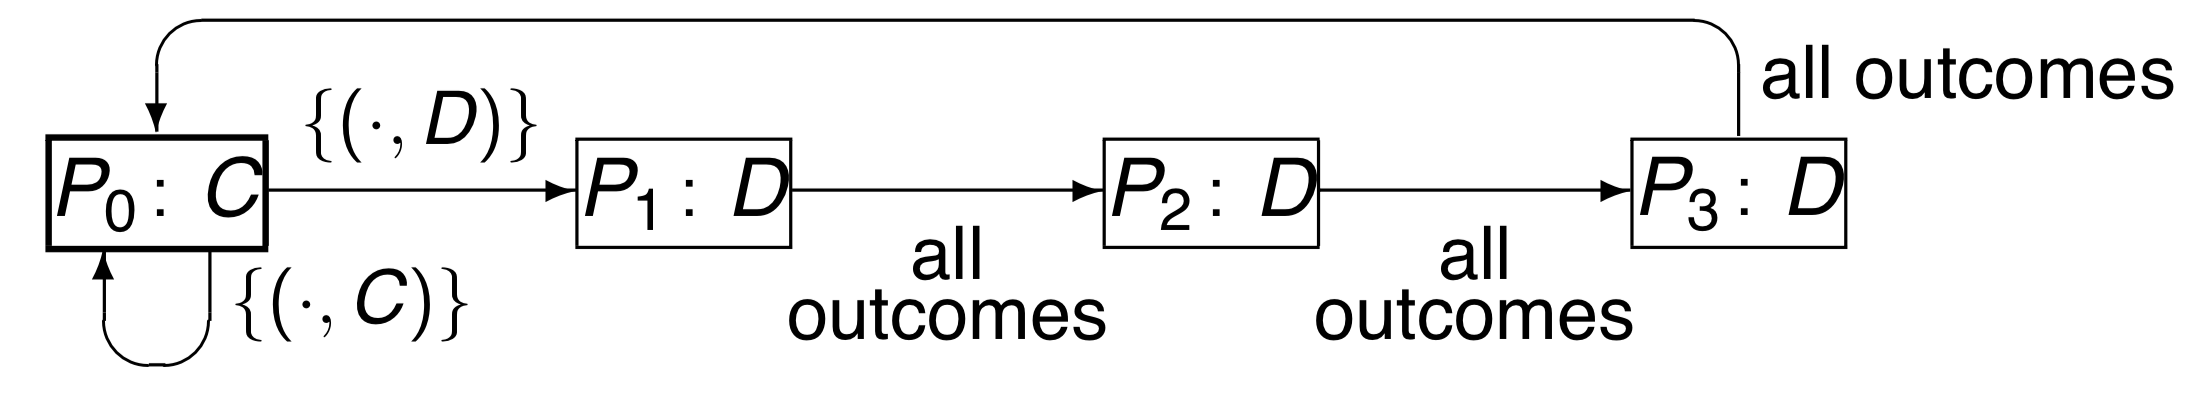
\includegraphics[width=0.7\linewidth]{fig/3punishment.png}
						\caption{Three period punishment strategy as an automaton.}
					\end{figure}
					\begin{proposition}[Generalized Limited Punishment, \textbf{$p$-Period Punishment}]
						The $p$-period punishment strategy is defined with $s_i^*(\varnothing) = C$, and if at time period $k$, $a_{-i}^k = D$, then the player play $D$ for the next $p$ periods as punishment no matter what action the opponent plays during the punishment. And then the player plays $C$ again beginning at time period $t=k+p+1$.
						\begin{proof}
							For the deviation \emph{not} to be profitable, we need
							\begin{align}
								&\delta^{k-1} y + \sum_{t=k+1}^{k+p} \delta^{t-1} 1 \leq \delta^{k-1} x + \sum_{t=k+1}^{k+p} \delta^{t-1} x \\
								&\iff \delta^{k-1} y \leq \delta^{k-1} x + \frac{(x-1)\delta^k (1 - \delta^p)}{1 - \delta} \\
								&\iff (y - x)\leq + \frac{\delta(1 - \delta^p)}{1 - \delta}(x - 1)
							\end{align}
						\end{proof}
					\end{proposition}
					
					\begin{proposition}
						For any value of $k \geq 1$, \emph{strategy pair} in which each player punishes other for $k$ periods in event of deviation is Nash equilibrium of infinitely repeated game if $\delta$ is \emph{close enough to 1}. The large $k$ is, the \emph{smaller lower bound on $\delta$}, that's, the \emph{mutually desirable outcome} $(C,C)$ is sustained by short punishment only if players are relatively patient.
					\end{proposition}
					
	\section{Lecture 9 Mar. 18 2019\\Bayesian Games}
		\subsection{Introduction}
			\begin{remark}
				Bayesian games allow players to face \ul{uncertainty about other players' preferences}.
			\end{remark}
			
			\begin{definition}[Informal Definition]
				A \textbf{Bayesian game}, $G^*$, consists a set of players, $N$, and action set $A_i$ for each player $i \in N$. Also a set of states of world, $\Omega$. Each player has a \textbf{prior belief} $p_i$, which is a probability distribution on $\Omega$.
				In each play of $G^*$, one state $\omega \in \Omega$ is realized, and each player $i$ receive a \textbf{signal} from his \textbf{signal function} $t_i = \tau_i(\omega) \in T_i$, this is referred as the \textbf{type} of player $i$. $T_i$ is the set of all possible types of player $i$. With $\tau_i(\omega)$ received (player $i$ does not actually observe $\omega$), player $i$ deduces that the actual state realized, $\omega$, is in the set $\tau_i^{-1}(t_i)$. This deduction provides player $i$'s \textbf{posterior belief} distribution on $\Omega$. For each $\omega \in \Omega$, the posterior belief of it is the probability of $\omega$, \emph{conditioned on $\tau_i(\omega) = t_i$}.
				\begin{equation}
					p_i(\omega|t_i) := \begin{cases}
						\frac{p_i(\omega)}{p_i(\tau_i^{-1}(t_i))} &\tx{ if } \omega \in \tau_i^{-1}(t_i) \\
						0 &\tx{ otherwise}
					\end{cases}
				\end{equation}
				For the conditional probability to make sense, we assume $p_i(\tau_i^{-1}(t_i)) > 0\ \forall t_i \in T_i$. Since a player in $G^*$ may be uncertain about which pair $(a, \omega)$ will be realized, so players' preference relations are defined over \emph{lottery} on $A \times \Omega$.
			\end{definition}
			
			\begin{definition}[Informal Definition]
				A \textbf{Bayesian equilibrium} is a strategy profile where \hl{each type of each player} ($\prod_{i \in N} T_i$) is best responding given their \emph{posterior beliefs}.
			\end{definition}
			
			\begin{remark}[Complication on Belief System]
				Here we assume individuals have \hl{exogenous beliefs}. In more complicated models, beliefs are endogenous, and beliefs change based on \emph{other players' (previous) actions}, and beliefs can be \emph{updated iteratively} in multi-period games.
			\end{remark}
		
		\subsection{Formal Definitions}
			\begin{definition}[Bayesian Game] A \textbf{Bayesian Game}, $G^* = \langle N, \Omega, (A_i), (T_i), (\tau_i), (p_i), (\pref_i) \rangle$, consists of
				\begin{enumerate}[(i)]
					\item A finite \textbf{player} set $N$;
					\item A set of \textbf{states} $\Omega$. Each $\omega \in \Omega$ represents one realization determines \emph{players' types}, \ul{$\Omega$ is assumed to be known by all players};
					\item For each player $i \in N$:
					\begin{enumerate}[(a)]
						\item An \textbf{action} set $A_i$;
						\item a set of \textbf{types (signals)} $T_i$;
						\item a \textbf{signal function} $\tau_i: \Omega \to T_i$ that associates a type(signal) with each state;
						\item A probability measure $p_i$ on $\Omega$ with $p_i(\tau_i^{-1}(t_i)) > 0\ \forall t_i \in T_i$, called player $i's$ \textbf{prior belief};
						\item For each $t_i \in T_i$ we can derive a \textbf{posterior belief} (distribution conditioned on $t_i = t_i$) function $\pi_i(\omega|t_i)$ or $\pi_i(t_{-i}|t_i)$, which can be expressed as a probability distribution on $\Omega$;
						\item A \textbf{preference relation} over probability distribution over $A \times \Omega$. And it's corresponding \textbf{payoff} $u_i(a_i, a_{-i}, t_i, t_{-i})$, and here \ul{we may assume $u_i$ does \emph{not} depend on $t_i$}.
					\end{enumerate}
				\end{enumerate}
			\end{definition}
			
			\begin{remark}
				The above definition allows the players to have different \emph{prior beliefs}. These beliefs may be related; \emph{commonly they are identical, coincident with an objective measure}.
			\end{remark}
			
			\begin{definition}[Strategy]
				A (mixed) \textbf{strategy}\footnote{This also covers the \emph{pure strategy} case since any pure strategy can be considered as a \emph{degenerate} mixed strategy.} for player $i$ in a Bayesian game is a function defined on $T_i$
				\begin{equation}
					\sigma_i: T_i \to \Delta(A_i)
				\end{equation}
				where $\sigma_i(a_i|t_i)$ denotes the chance of player $i$ playing $a_i$ given this player is in type $t_i$.
			\end{definition}
			
			\begin{remark}[Interpretation]
				For a player $i$ in a Bayesian game, one strategy assigns a probability distribution over his action set \ul{for each $t_i \in T_i$}.
			\end{remark}
			
			\begin{definition}
				The \textbf{expected payoff}, given player $i$ is type $t_i$ and conditioned on player $i$'s own belief $\pi_i$, from action $a_i$ is 
				\begin{gather}
					U_i(a_i, \sigma_{-i}| t_i) 
					= \sum_{\omega \in \Omega} u_i(a_i, \sigma_{-i}(\omega)|t_i)\pi_i(\omega|t_i) \\
					= \int_{\Omega} u_i(a_i, \sigma_{-i}(\omega)|t_i)\ d\pi_i(\omega|t_i)
				\end{gather}
			\end{definition}
			
			\begin{definition}
				An action $a_i \in A_i$ is a \textbf{best response} to $\sigma_i$, given player type $t_i$, if
				\begin{equation}
					U_i(a_i, \sigma_{-i}|t_i) \geq U_i(\tilde{a}_i, \sigma_{-i}|t_i)\ \forall \tilde{a}_i \in A_i
				\end{equation}
				\emph{The definition for a mixed strategy $\sigma_i \in \Delta(A_i)$ is similar}.
			\end{definition}
			
			\begin{definition}
				A Bayesian Nash equilibrium is a strategy profile for each player such that the strategy for \hl{each type} of \hl{each player} is a best response \ul{given the strategies for the other players deduced from the signal received}.
			\end{definition}
			
			\begin{definition}[Lottery Generated by a Bayesian Game]
				The posterior belief of player $i$, together with an action profile $a^*$ in $G^*$, generates a lottery $L_i(a^*, t_i)$ over $A \times \Omega$: the probability assigned by $L_i(a^*, t_i)$ to 
				\begin{equation}
					\Big((a^*(j, \tau_j(\omega)))_{j\in N}, \omega \Big)
				\end{equation}
				is the \emph{posterior belief} that the state is $\omega$ when he receives the signal $t_i$ and $a^*(j, \tau_j(\omega))$ being the action of player $(j, \tau_j(\omega))$ for each $j \in N$ in the profile $a^*$.
			\end{definition}
			
			\begin{definition}[Formal Definition]
				A \textbf{Nash equilibrium of a Bayesian Game}, \\$\langle N, \Omega, (A_i), (T_i), (\tau_i), (p_i), (\pref_i) \rangle$ is a Nash equilibrium of the strategic game defined as follows.
				\begin{itemize}
					\item The set of players is the set of all pairs $(i, t_i)$ for $i \in N$ and $t_i \in T_i$.
					\item The set of actions of each player $(i, t_i)$ is $A_i$.
					\item The preference ordering $\pref^*_(i, t_i)$ of each player $(i, t_i)$ is defined by
					\begin{equation}
						a^* \pref^*_{(i, t_i)} b^* \iff L_i(a^*, t_i) \pref_i L_i(b^*, t_i)
					\end{equation}
					where $L_i(a^*, t_i)$ is the lottery over $A \times \Omega$ that assigns probability
					$
						\frac{p_i(\omega)}{p_i(\tau_i^{-1}(\omega))}
					$
					to $(a^*(j, \tau_j(\omega)))_{j\in N}$ if $\omega \in \tau_i^{-1}(t_i)$, zero otherwise.
				\end{itemize}
			\end{definition}
\end{document}




























